\documentclass[letterpaper, 12pt]{article}
\usepackage[margin=1in]{geometry}
\usepackage{amsmath}
\usepackage{amssymb}
\usepackage{xcolor}
\usepackage{graphicx}
\usepackage[center]{caption}
\usepackage{hyperref}
\usepackage{fancyhdr}

\pagestyle{fancy}
\fancyhf{}
\rhead{
    Shendong Li
    Calc 1
}
\rfoot{
    Page \thepage
}

\usepackage{indentfirst}
\setlength{\parindent}{2em}

\begin{document}
\title{Response to Maggie Bao}
\author{by Shengdong Li}
\date{18 April 2020}
\maketitle
\section{Intro}
Hello Maggie! What a beautiful mug that you have! The rich, golden potato coloring on the top top of the mug contrasts exquisitely with the healthy avocado paste on the rest of body. It really reminds me of a reverse-ice cream cone.
\section{Solution}
I first tried to represent the base of the mug by graphing it on Desmos, to better visualize the problem. I also made this problem a $dy$ problem because I felt that it would be slightly more intuitive to do.
\begin{figure}[h]
    \begin{center}
        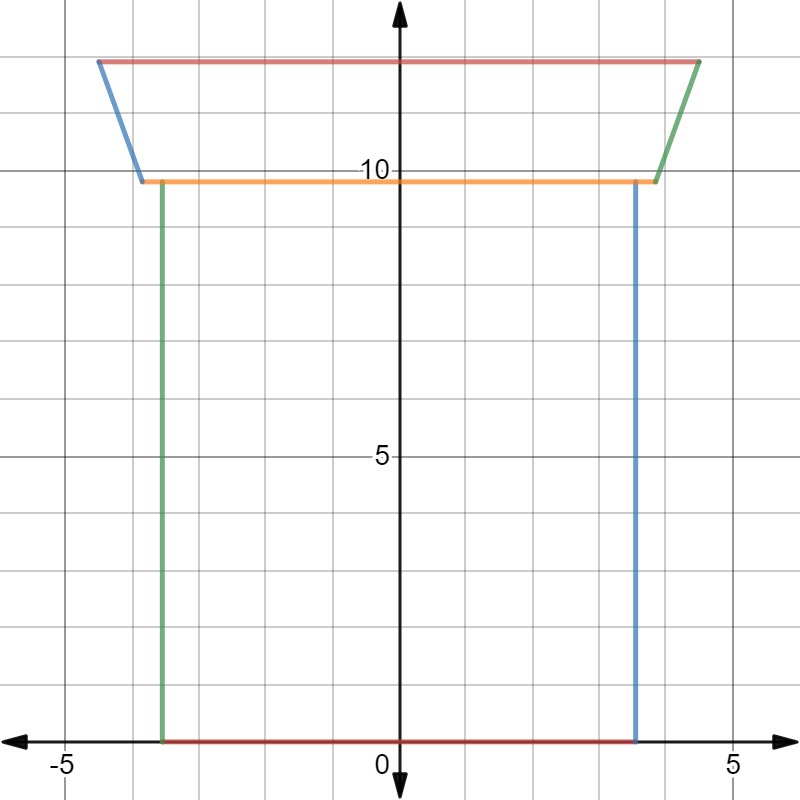
\includegraphics[scale=.3]{mug.png}
        \caption{\textit{Cool mug.} Desmos link \href{https://www.desmos.com/calculator/ms6wz8unq4}{\textcolor{blue}{here}}, also see embed below}
    \end{center}
\end{figure}
\begin{align}
    \intertext{First, we'll find the volume of the rectangular prism. Let's define the $A(x)$ function in terms of $b$}
    A(b)\:of\:square                         & = b^2
    \intertext{Our $x$ is defined by the two functions $x=3.55$ and $x=-3.55$}
    x                                        & = 3.55-(-3.55)                                                                    \\
                                             & =7.1
    \intertext{Now we can make our area function in terms of $y$ (kind of)}
    A(y)                                     & =(7.1)^2                                                                          \\
                                             & =\boxed{50.41}
    \intertext{As defined by the problem, our bottom bound is $0$ and our top bound is $9.8$}
    a                                        & = \boxed{0}                                                                       \\
    b                                        & = \boxed{9.8}
    \intertext{Now integrate the area function within the defined ranges to find the volume of the prism}
    \int_{a}^{b}A\left(y\right)dy            & =\int_{0}^{9.8}\left(50.41\right)dy                                               \\
                                             & =50.41y\Big|_{0}^{9.8}                                                            \\
                                             & =50.41\left(9.8\right)-50.41\left(0\right)                                        \\
                                             & =50.41\left(9.8\right)                                                            \\
                                             & =\boxed{494.018\:cm^3}
    \intertext{Moving onto the cylindrical frustrum, first define the area function of the cross-sections perpendicular to the $y-axis$ in terms of $r$}
    A(r)                                     & =\pi r^2
    \intertext{$r$ is actually just one side of one of our linear functions}
    r                                        & =\frac{13}{42}y+\frac{49}{60}
    \intertext{Now we can make our area function in terms of $y$}
    A(y)                                     & =\boxed{\pi(\frac{13}{42}y+\frac{49}{60})^2}
    \intertext{As defined by the problem, the bottom bound is $9.8$ and the top bound is $11.9$}
    a                                        & =\boxed{9.8}                                                                      \\
    b                                        & =\boxed{11.9}
    \intertext{Now we can integrate the area function from within the defined ranges to find the volume of the frustrum}
    \int_{a}^{b}A\left(y\right)dy            & =\int_{9.8}^{11.9}\left(\pi\left(\frac{13}{42}y+\frac{49}{60}\right)^{2}\right)dy \\
                                             & =\pi\int_{9.8}^{11.9}\left(\left(\frac{13}{42}y+\frac{49}{60}\right)^{2}\right)dy
    \intertext{$U-sub$ might make the problem slightly cleaner}
    u                                        & = \frac{13}{42}y+\frac{49}{60}                                                    \\
    du                                       & =\frac{13}{42} dx                                                                 \\
    \frac{42}{13}du                          & = dx
    \intertext{Update the ranges}
    a                                        & =\frac{13}{42}\left(11.9\right)+\frac{49}{60}                                     \\
                                             & =4.5                                                                              \\
    b                                        & =\frac{13}{42}\left(9.8\right)+\frac{49}{60}                                      \\
                                             & =3.85
    \intertext{Substitute and integrate!}
    \frac{42}{13}\pi\int_{3.85}^{4.5}u^{2}du & =\frac{42}{13}\pi\left(\frac{u^{3}}{3}\right)\Big|_{3.85}^{4.5}                   \\
                                             & =\frac{42}{39}\pi\left(u^3\right)\Big|_{3.85}^{4.5}                               \\
                                             & =\frac{42}{39}\pi\left(\left(4.5\right)^{3}-\left(3.85\right)^{3}\right)          \\
                                             & =\frac{42}{39}\pi\left(34.058375\right)                                           \\
                                             & =\boxed{115.228...\:cm^3}
    \intertext{Now we just add the area of the prism to the area of our frustrum to get the total volume of the mug}
    115.228...+494.018                       & \approx\boxed{609.25\:cm^3}
\end{align}
\section{Conclusion}
I think that doing your word problem reminded me how it isn't always best to distribute factors or squares because $u$-sub can make the problem a lot cleaner and save some time. (Speaking of time if you still have some time pls do my problem no one wants to do my problem thx)
\end{document}